\documentclass[border=6pt]{standalone}
\usepackage{amsmath,amssymb}
\usepackage{tikz}
\usetikzlibrary{arrows.meta,shadows,calc,backgrounds}
\begin{document}
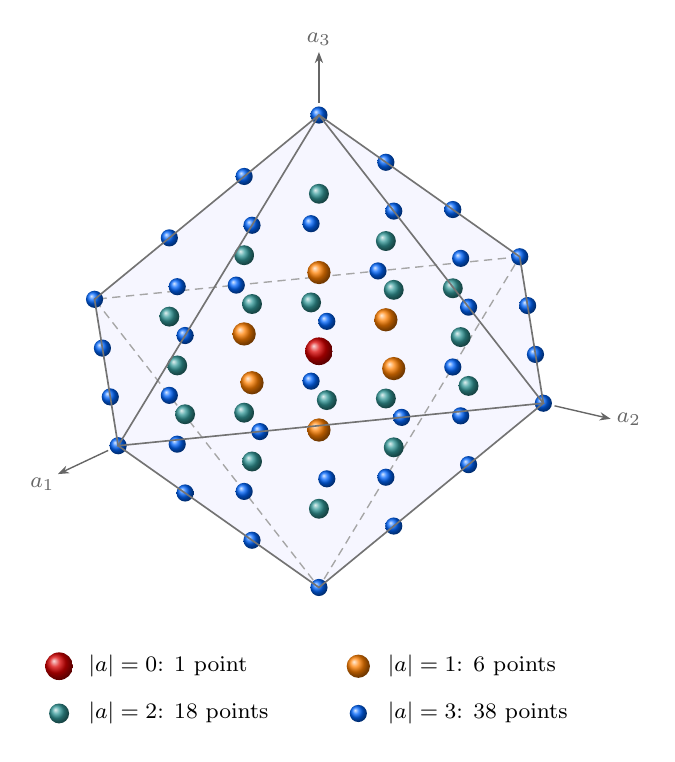
\begin{tikzpicture}[x={(-0.85cm,-0.40cm)},y={(0.95cm,-0.22cm)},z={(0cm,1.0cm)},
  lab/.style={font=\footnotesize},
  edge/.style={line width=0.6pt,black!55},
  hidden/.style={line width=0.5pt,black!35,dash pattern=on 3pt off 2pt},
  face/.style={fill=blue!45,fill opacity=0.08,draw=none}]
% the octahedron |a_1|+|a_2|+|a_3| <= 3 seen from the octant (+,+,+):
% the edges around the face of the octant (-,-,-) are hidden
\begin{scope}[on background layer]
  \foreach \sx/\sy/\sz in {3/3/3,3/3/-3,3/-3/3,-3/3/3}
    { \fill[face] (\sx,0,0) -- (0,\sy,0) -- (0,0,\sz) -- cycle; }
  \draw[hidden] (-3,0,0) -- (0,-3,0) -- (0,0,-3) -- cycle;
\end{scope}
% the 63 points, from back to front
\foreach \x/\y/\z/\r in {
    -3/0/0/3, -2/-1/0/3, -1/-2/0/3, 0/-3/0/3, -2/0/-1/3, -1/-1/-1/3, 0/-2/-1/3, -1/0/-2/3,
    0/-1/-2/3, -2/0/0/2, -1/-1/0/2, 0/0/-3/3, 0/-2/0/2, -1/0/-1/2, 0/-1/-1/2, -2/0/1/3,
    -1/-1/1/3, 0/0/-2/2, 0/-2/1/3, -2/1/0/3, -1/0/0/1, 0/-1/0/1, 1/-2/0/3, -1/1/-1/3,
    0/0/-1/1, 1/-1/-1/3, -1/0/1/2, 0/1/-2/3, 0/-1/1/2, 1/0/-2/3, -1/1/0/2, 0/0/0/0, 1/-1/0/2,
    -1/0/2/3, 0/1/-1/2, 0/-1/2/3, 1/0/-1/2, -1/1/1/3, 0/0/1/1, 1/-1/1/3, -1/2/0/3, 0/1/0/1,
    1/0/0/1, 2/-1/0/3, 0/2/-1/3, 0/0/2/2, 1/1/-1/3, 2/0/-1/3, 0/1/1/2, 1/0/1/2, 0/2/0/2,
    0/0/3/3, 1/1/0/2, 2/0/0/2, 0/1/2/3, 1/0/2/3, 0/2/1/3, 1/1/1/3, 2/0/1/3, 0/3/0/3, 1/2/0/3,
    2/1/0/3, 3/0/0/3} {
  \ifcase\r
    \shade[ball color=red!85!black] (\x,\y,\z) circle (5pt);
  \or
    \shade[ball color=orange] (\x,\y,\z) circle (4.2pt);
  \or
    \shade[ball color=teal!80] (\x,\y,\z) circle (3.6pt);
  \or
    \shade[ball color=blue!60!cyan] (\x,\y,\z) circle (3.1pt);
  \fi
}
\draw[edge] (3,0,0) -- (0,3,0) -- (0,0,3) -- cycle;
\draw[edge] (3,0,0) -- (0,-3,0) -- (0,0,3);
\draw[edge] (3,0,0) -- (0,0,-3) -- (0,3,0);
\draw[edge] (0,0,3) -- (-3,0,0) -- (0,3,0);
% the axes through the centre
\draw[-{Stealth[length=4pt]},line width=0.5pt,black!60] (3.15,0,0) -- (3.9,0,0) node[lab,anchor=north east,inner sep=1pt] {$a_1$};
\draw[-{Stealth[length=4pt]},line width=0.5pt,black!60] (0,3.15,0) -- (0,3.9,0) node[lab,anchor=west,inner sep=2pt] {$a_2$};
\draw[-{Stealth[length=4pt]},line width=0.5pt,black!60] (0,0,3.15) -- (0,0,3.8) node[lab,anchor=south,inner sep=2pt] {$a_3$};
% legend
\foreach \c/\s/\t/\y/\xx in {red!85!black/5/{$|a|=0$: $1$ point}/-4.0/-3.3, orange/4.2/{$|a|=1$: $6$ points}/-4.0/0.5,
    teal!80/3.6/{$|a|=2$: $18$ points}/-4.6/-3.3, blue!60!cyan/3.1/{$|a|=3$: $38$ points}/-4.6/0.5} {
  \shade[ball color=\c] (canvas cs:x=\xx cm,y=\y cm) circle (\s pt);
  \node[lab,anchor=west] at (canvas cs:x=\xx cm+0.25cm,y=\y cm) {\t};
}
\end{tikzpicture}
\end{document}
